%%%%%%%%%%%%%%%%%%%%%%%%%%%%%%%%%%%%%%%%%%%%%%%%%%%%%%%%%%%%%%%%%%%%%%%%%%%%%%%%%%
%%% Navigation
%%% 
%%%
%%%%%%%%%%%%%%%%%%%%%%%%%%%%%%%%%%%%%%%%%%%%%%%%%%%%%%%%%%%%%%%%%%%%%%%%%%%%%%%%%%
\chapter{Navigation Results} \label{ch:results_navigation}

% The structure of this chapter needs revision.

% What do we have to talk about here?
% Well, I suppose the point of this chapter is to present how well the algorithm worked.
% What is there to present?
% I suppose it should be shown that the algorithm does indeed nav the robot,
% as that is not necessarily assumed in the chapter explaining the navigation.
% Some things you might want to know:
% Qualitatively, how well did it nav the robot?

% Ok, so what can I show?
% I can show pictures of the Nao naving around different environments getting to goals
% I can show what the robot thought his pose was based on the goal.
% I can list the optimal parameters for naving.
% I wish I could have shown laser data, because maybe I could have shown a potential field map.
% Can I show the different parts of what the nav was using? No, because the straight line planner
% and escape strategy was not implemented.

\section{Intro/Experimental Setup}
As mentioned in Chapter \ref{ch:platform}, in order to test the GOZILA algorithm,
the Nao was used, and had a Hokuyo LIDAR stuck to its chest.
We used Nao's built in walking to walk, which as we'll discuss, sucked (put us at a disadvantage),
because since we strapped a big mass to it's chest that it didn't know about,
the thing had a tendency to loose stability and fall over.
(In fact we couldn't keep going because the fucker kept falling over and breaking it's gears.)

The LIDAR allowed the Nao to detect obstacles. These LIDAR points fed the algorithm and repelled.

Also, since we needed to know where the goal was we used the built it blob
detection on Nao and made up a big red cube for it to detect.
The stock blob detection not only gives you bearing to a goal but it also assumes that the
red blob is a certain size (diameter: 0.06 m) and therefore can estimate range to the obstacle.
While you would think then that we should have used an object that size,
since we were asking it to track something so far away and cameras suck, we had to use a bigger (0.127 m or 5 inch
side length or twice as big)
object so it could be seen at distance.
This of course then meant that the range measurement was incorrect, but since we were
only using the range measurement for the goal attraction and to determine when to stop,
it wasn't that big of a deal and we could tune around it.
Now that I think about it, what we should have done was calibrate the distance with this
object so the tuning for GODZILA and the stopping distance would be ``real'' and not to
this messed up thing.
You would definitely definitely definitely have to do this if you were going to do mapping,
which was the next step.

The outer perimeter of the arena way yay big. The LIDAR range was 5 meters, so having the
perimeter, which was all straight flat walls, meant that the robot could always see them.
This let things be consistent when testing, thought not strictly necessary for the algorithm to
work as the robot doesn't need to localize in order to navigate.
You don't see these walls in the figures, for aesthetic reasons.

Hey! Also! The whole thing was recorded with a global camera (A GoPro).
Having a fixed camera like this is good because it makes tracking the robot
to measure it's performance trivial.
We used some image processing to track the Nao's orangeness, clustered to
find the Nao-like things that were being tracked in the image,
and then fit a 5th order polynomial curve to it to estimate the path of the
robot.

All in all, you can see that the robot makes it to the goal.
It has a hard time in some places, but this isn't because of the algorithm,
it's because of the balance issues with the LIDAR and the walking.
You can see this a lot in the narrow example on the left side of the aperture where the
robot oscillates a lot, but in general you can see a periodic amplitude (?) thoughout 
the entire gait which is not normal to the walking gait and being caused by the
instability introduced (though obviously there is some normal amount of periodicity
to any walking gait but it shouldn't be THAT bad).

Somewhere we should mention that this method only works if the shape of the field is
convex. The potential field method is subject to local minima (the U-shape mentioned in Chapter
\ref{ch:navigaiton} is a good example). It would be the job of the escape strategy to
try and break out of this.

The escape strategy is a bit tough because detecting ``stuckedness'' is tough in long
limit cycles without mapping.
In local minima that cause the robot to more or less stop, you can try and detect that
the distance to the goal hasn't reduced in awhile.
This was mentioned in Chapter \ref{subsec:escape_strategy}.

\subsection{Ok, so then where did we test this?}
We did three different environments with different environmental features.
So, as a control basically, one of the environments was just open. Yes there are walls
so there is a repulsive force but nothing should be obstructing the attraction to the
goal and if this doesn't work then something is really messed up. Figure \ref{fig:nav_open_setup1}
shows the setup.

\begin{figure}
  \includegraphics[width=\textwidth]{nav/open/no_path/frame1.png}
  \caption{Here's the open arena. Robot on left. Goal is the red boxy thing on the right.
           There's a bunch of walls that the robot can also see. Those same walls will
           always be there in all of the setups.}
  \label{fig:nav_open_setup1}
\end{figure}

Next we tried one that had a narrow opening between the robot and the goal.
The aperture is about 73 cm wide.
This aperture is about 2.6 times the width of the body of the robot (27.5 cm wide).
It was more or less the
limit of this approach because if we allow the robot to get closer to obstacles it tends
to cut too close to corners and other things and mess up.
To solve this, you'd need something that plans paths though these narrow but traversable
areas and have intermediate goals along this path for GODZILA to use.
These would then ``pull'' the robot through the narrow aperture.
This is how the straight line planner works when the goal is in sight.
That's not the case in the setup so the straight line planner cannot be invoked.
Also, that's again not really the focus of this algorithm and as mentioned in
Chapter \ref{ch:navigation}, the responsibility of some global planner.
Figure \ref{fig:nav_narrow_setup1} shows the setup.

\begin{figure}
  \includegraphics[width=\textwidth]{nav/narrow/no_path/frame1.png}
  \caption{Here's the arena with the narrow opening.
           The opening is about 2.6 times the width of the robot.
           This is pretty much the minimum aperture width this method can allow.}
  \label{fig:nav_narrow_setup1}
\end{figure}

Finally, we invoked a more complicated geometry where the robot had to go around
a large obstacle. In this case, the robot is always relatively close to obstacles and the
being pushed. Despite the constant repulsion, the goal is attractive enough to
pull the robot to the goal. Figure \ref{fig:nav_square_setup1} shows the setup.

\begin{figure}
  \includegraphics[width=\textwidth]{nav/square/no_path/frame1.png}
  \caption{This is the arena with the large obstacle.
           In this case, there's an obstacle closer to the robot than the goal most of the time.
           The hallway is about as narrow as you can make it.}
  \label{fig:nav_square_setup1}
\end{figure}

\subsection{How was the test setup constructed?}
Everything was boxy since that was the easiest shape to put together that had the
same 2D projection throughout. We could only test things at laser height and obstacles
like chairs which can have things jutting out above and below the laser are obviously going
to mess things up because the robot can't see them, so there really wasn't a point to testing
that.
Maybe we could have had more thin objects but then we're talking about the laser resolution
constraint. This would probably be a good one to try next time since it falls in the range of
detectability though it's sort of now in the obstacle avoidance part of things
which should be it's own algorithm in the stack of things to do all of navigation.

The robot was told to stop 0.3 meters radius from the goal.

\section{Parameter stuff}
WHAT ARE THE OPTIMAL PARAMETERS/PARAMETERS USED.
Table \ref{tab:nav_params1} shows the parameters used.
This table will have to be reduced and most likely added to the appendix in it's
full form. Also, probably going to have to explain all of these parameters.
Probably something like, ``we interface with/tune the algorithm through the following parameter''
and then explain each one in relation to the math or whatever.

\begin{table}
  \centering
  \begin{tabularx}{0.65 \textwidth}{|X||X|}
    \hline
    \textbf{Configuration Parameter}  & \textbf{Minimum Angle (degrees)}\\  \hline\hline
    goalStoppingRadius        &   0.3   \\  \hline
    vmin                      &   -0.4  \\  \hline
    vmax                      &   0.4   \\  \hline
    wmin                      &  -0.2   \\  \hline
    wmax                      &   0.2   \\  \hline
    clearanceThreshold        &   0.3   \\  \hline
    obstacleThreshold         &   3     \\  \hline
    goalAttraction            &   100   \\  \hline
    obstacleRepulsionTurning  &   20    \\  \hline
    obstacleAttraction        &   0     \\  \hline
    obstacleGoalBearingRatio  &   1     \\  \hline
    vehicleInertia            &   15    \\  \hline
    velocityGain              &   5     \\  \hline
    obstacleRepulsionForward  &   5     \\  \hline
    angularRateBraking        &   3     \\  \hline
  \end{tabularx} 
  
  \caption{These are the parameters we used. They worked pretty well.}
  \label{tab:nav_params1}
\end{table}

\textbf{goalStoppingRadius}        \\
The radius at which the robot considers itself at the goal.

\textbf{clearanceThreshold} \\
Method for setting the minimum acceptable distance between the vehicle and an obstacle.
Setting this distance does not guarantee that the robot will never violate this threshold.
Distance from the center of the robot to the center of an obstacle in meters. 
This distance is center to center because all objects are modeled as points. \\

\textbf{obstacleThreshold}         \\
Method for setting the obstacle range at which it is acceptable to treat obstacles
as attractive rather than repulsive.
Obstacle range threshold measured in meters. \\

\textbf{TUNING ANGULAR} \\
Method for tuning the planning parameters for angular velocity. \\

\textbf{goalAttraction}            \\
Tunes the strength of goal attraction.
Larger values increase attraction strength. \\

\textbf{obstacleRepulsionTurning}  \\
Tunes the strength of obstacle repulsion for 
obstacles closer than the obstacle range threshold.
Larger values increase repulsion strength. \\

\textbf{obstacleAttraction}        \\
Tunes the strength of obstacle attraction for 
obstacles farther than the obstacle range threshold.
Larger values increase attraction strength. \\

\textbf{obstacleGoalBearingRatio}  \\
Tunes the trade off between avoiding obstacles 
which are in the vehicle's current direction 
of travel versus avoiding objects which are 
in the direction of the goal.
This parameters ranges from 1 to 0. 
Values closer to 1 amplify the avoidance of 
obstacles in the direction of travel.
Values closer to 0 amplify the avoidance of 
obstacles in the direction of the goal. \\

\textbf{vehicleInertia}            \\
Tunes the strength of the vehicle's resistance 
to turning. Larger values mean more resistance.

\textbf{TUNE LINEAR}
 Method for tuning the planning parameters for linear velocity.
\textbf{velocityGain}              \\
Tunes the aggressiveness of the linear velocity. 
Larger number produces more aggressiveness. \\

\textbf{obstacleRepulsionForward}  \\
Tunes the strength of obstacle repulsion.
Larger values increase repulsion strength.\\

\textbf{angularRateBraking}        \\
Tunes the amount by which high turning rates reduce linear velocity.
Larger values reduce linear velocity. \\


\section{Picture of the Nao navigating}

Basically, these pictures are here just to show you that the robot
made it through the environment. It's not strictly necessary but you wouldn't
believe me otherwise and they're pretty to look at.
For convenience, I overlaid the best fit path from the image analysis just
so you could see ``where'' Nao was going and to give continuity to what you
are looking at.

\begin{figure}
  \centerline{
    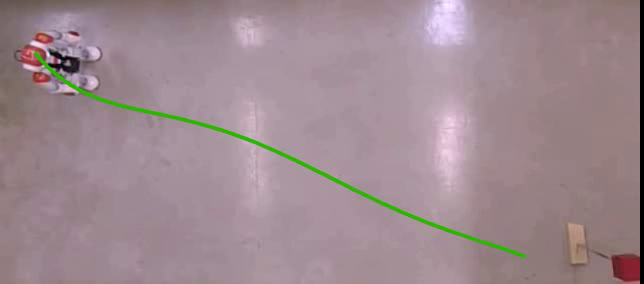
\includegraphics[width=0.5\textwidth]{nav/open/path/open_path1.png}
    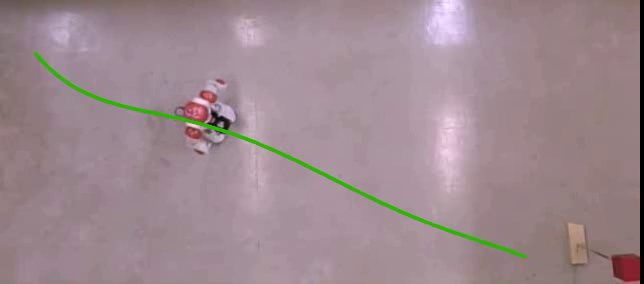
\includegraphics[width=0.5\textwidth]{nav/open/path/open_path2.png}
  }
  \vspace*{0.05in}
  \centerline{
    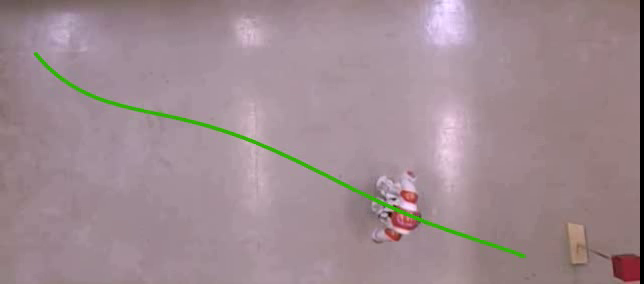
\includegraphics[width=0.5\textwidth]{nav/open/path/open_path3.png}
    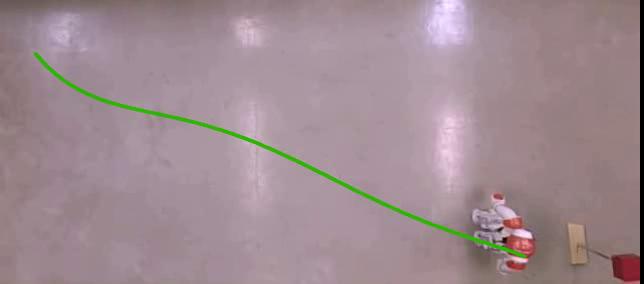
\includegraphics[width=0.5\textwidth]{nav/open/path/open_path4.png}
  }
  \caption{This guy shows the Nao walking to the goal in the open area.
           The robot basically walks in a straight line, which is what you'd expect.}
  \label{fig:nav_open_frames1}
  \vspace*{-0.07in}
\end{figure}

\begin{figure}
  \centerline{
    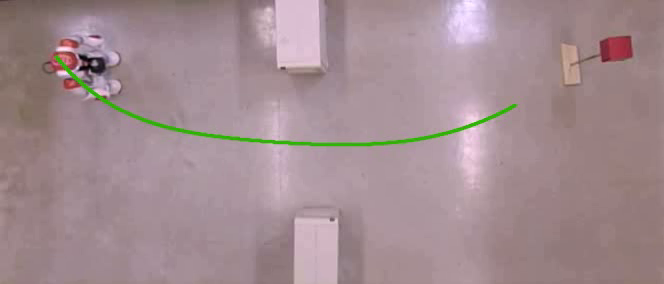
\includegraphics[width=0.5\textwidth]{nav/narrow/path/narrow_path1.png}
    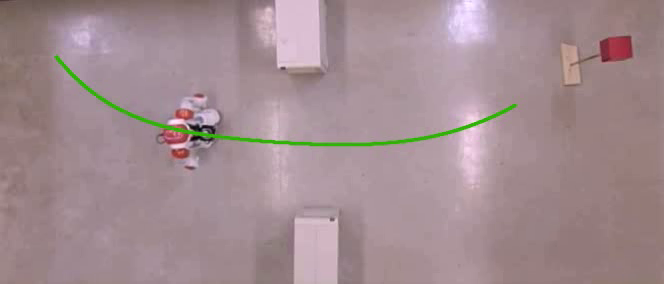
\includegraphics[width=0.5\textwidth]{nav/narrow/path/narrow_path2.png}
  }
  \vspace*{0.05in}
  \centerline{
    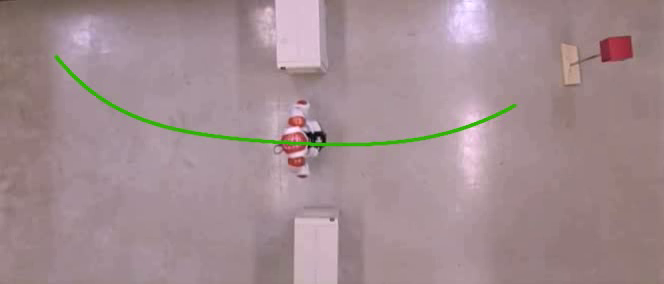
\includegraphics[width=0.5\textwidth]{nav/narrow/path/narrow_path3.png}
    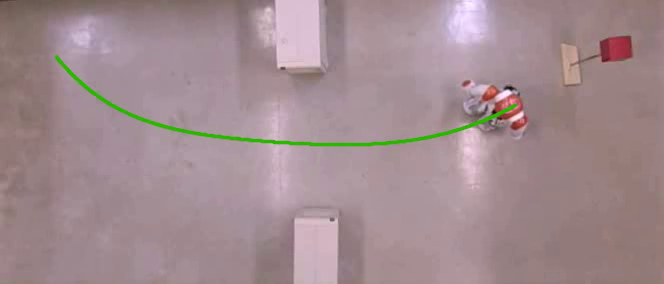
\includegraphics[width=0.5\textwidth]{nav/narrow/path/narrow_path4.png}
  }
    \caption{This one shows the robot walking through the narrow aperture.
             You can see that the robot walks more or less straight the the opening and then to the goal.}
    \label{fig:nav_narrow_frames1}
        \vspace*{-0.07in}
\end{figure}

\begin{figure}
  \centerline{
    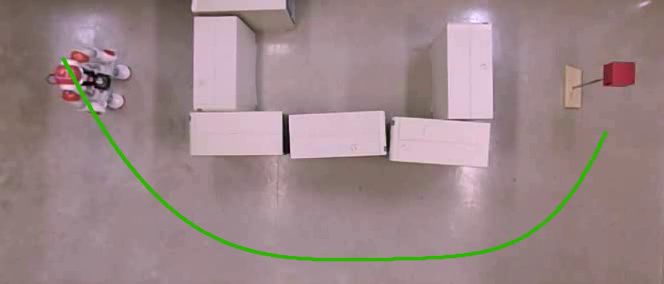
\includegraphics[width=0.5\textwidth]{nav/square/path/square_path1.png}
    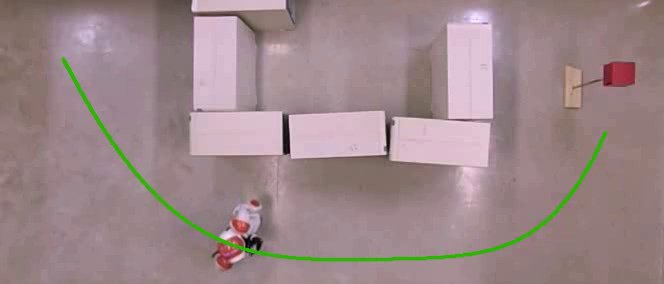
\includegraphics[width=0.5\textwidth]{nav/square/path/square_path2.png}
  }
  \vspace*{0.05in}
  \centerline{
    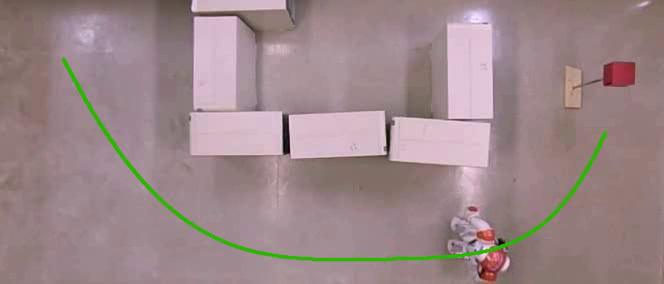
\includegraphics[width=0.5\textwidth]{nav/square/path/square_path3.png}
    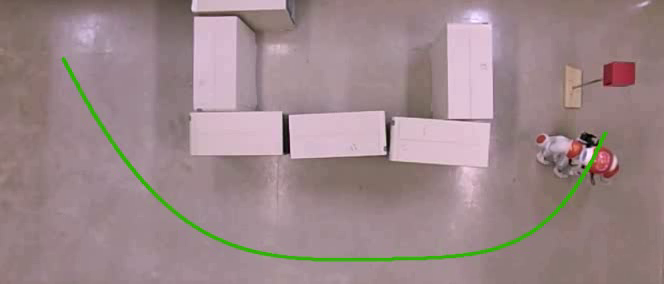
\includegraphics[width=0.5\textwidth]{nav/square/path/square_path4.png}
  }
    \caption{This figure shows the robot walking around a large obstacle.
             The robot walks down the corridor to the goal.}
    \label{fig:nav_square_frames1}
        \vspace*{-0.07in}
\end{figure}

\section{The plots from the global camera tracking}
These are what comes out of the image processing.
I guess I should tell you that I used OpenCV to do blob tracking, some dilations, near cluster
joining (like the head and shoulders show up as 3 orange blobs so they are joined to estimate the
center of the robot), then density based clustering to see which ones belong to which (the red cube is
orange enough to register as something to track so instead of trying to tune the fuck out of the colors
or use some other technique like template-matching or something I don't know about yet since I'm just 
starting to use OpenCV), I opted to do clustering and then I manually select which cluster of points are
the Nao's. Then I used a 5th order polynomial to fit the path.

Again, I'm not really sure why you need to see this other than to say here's an analysis of 
what the robot did that's a little more than just straight pictures.
You can really see the periodicity in the gait on these graphs.

You should notice here that while the robot was told to stop at 0.3 m, it actually
stops closer to 0.8 m from the goal.
This is because of the mismatch between how big the robot thinks the red object is
and the fact that it's about twice as big.

\begin{figure}
  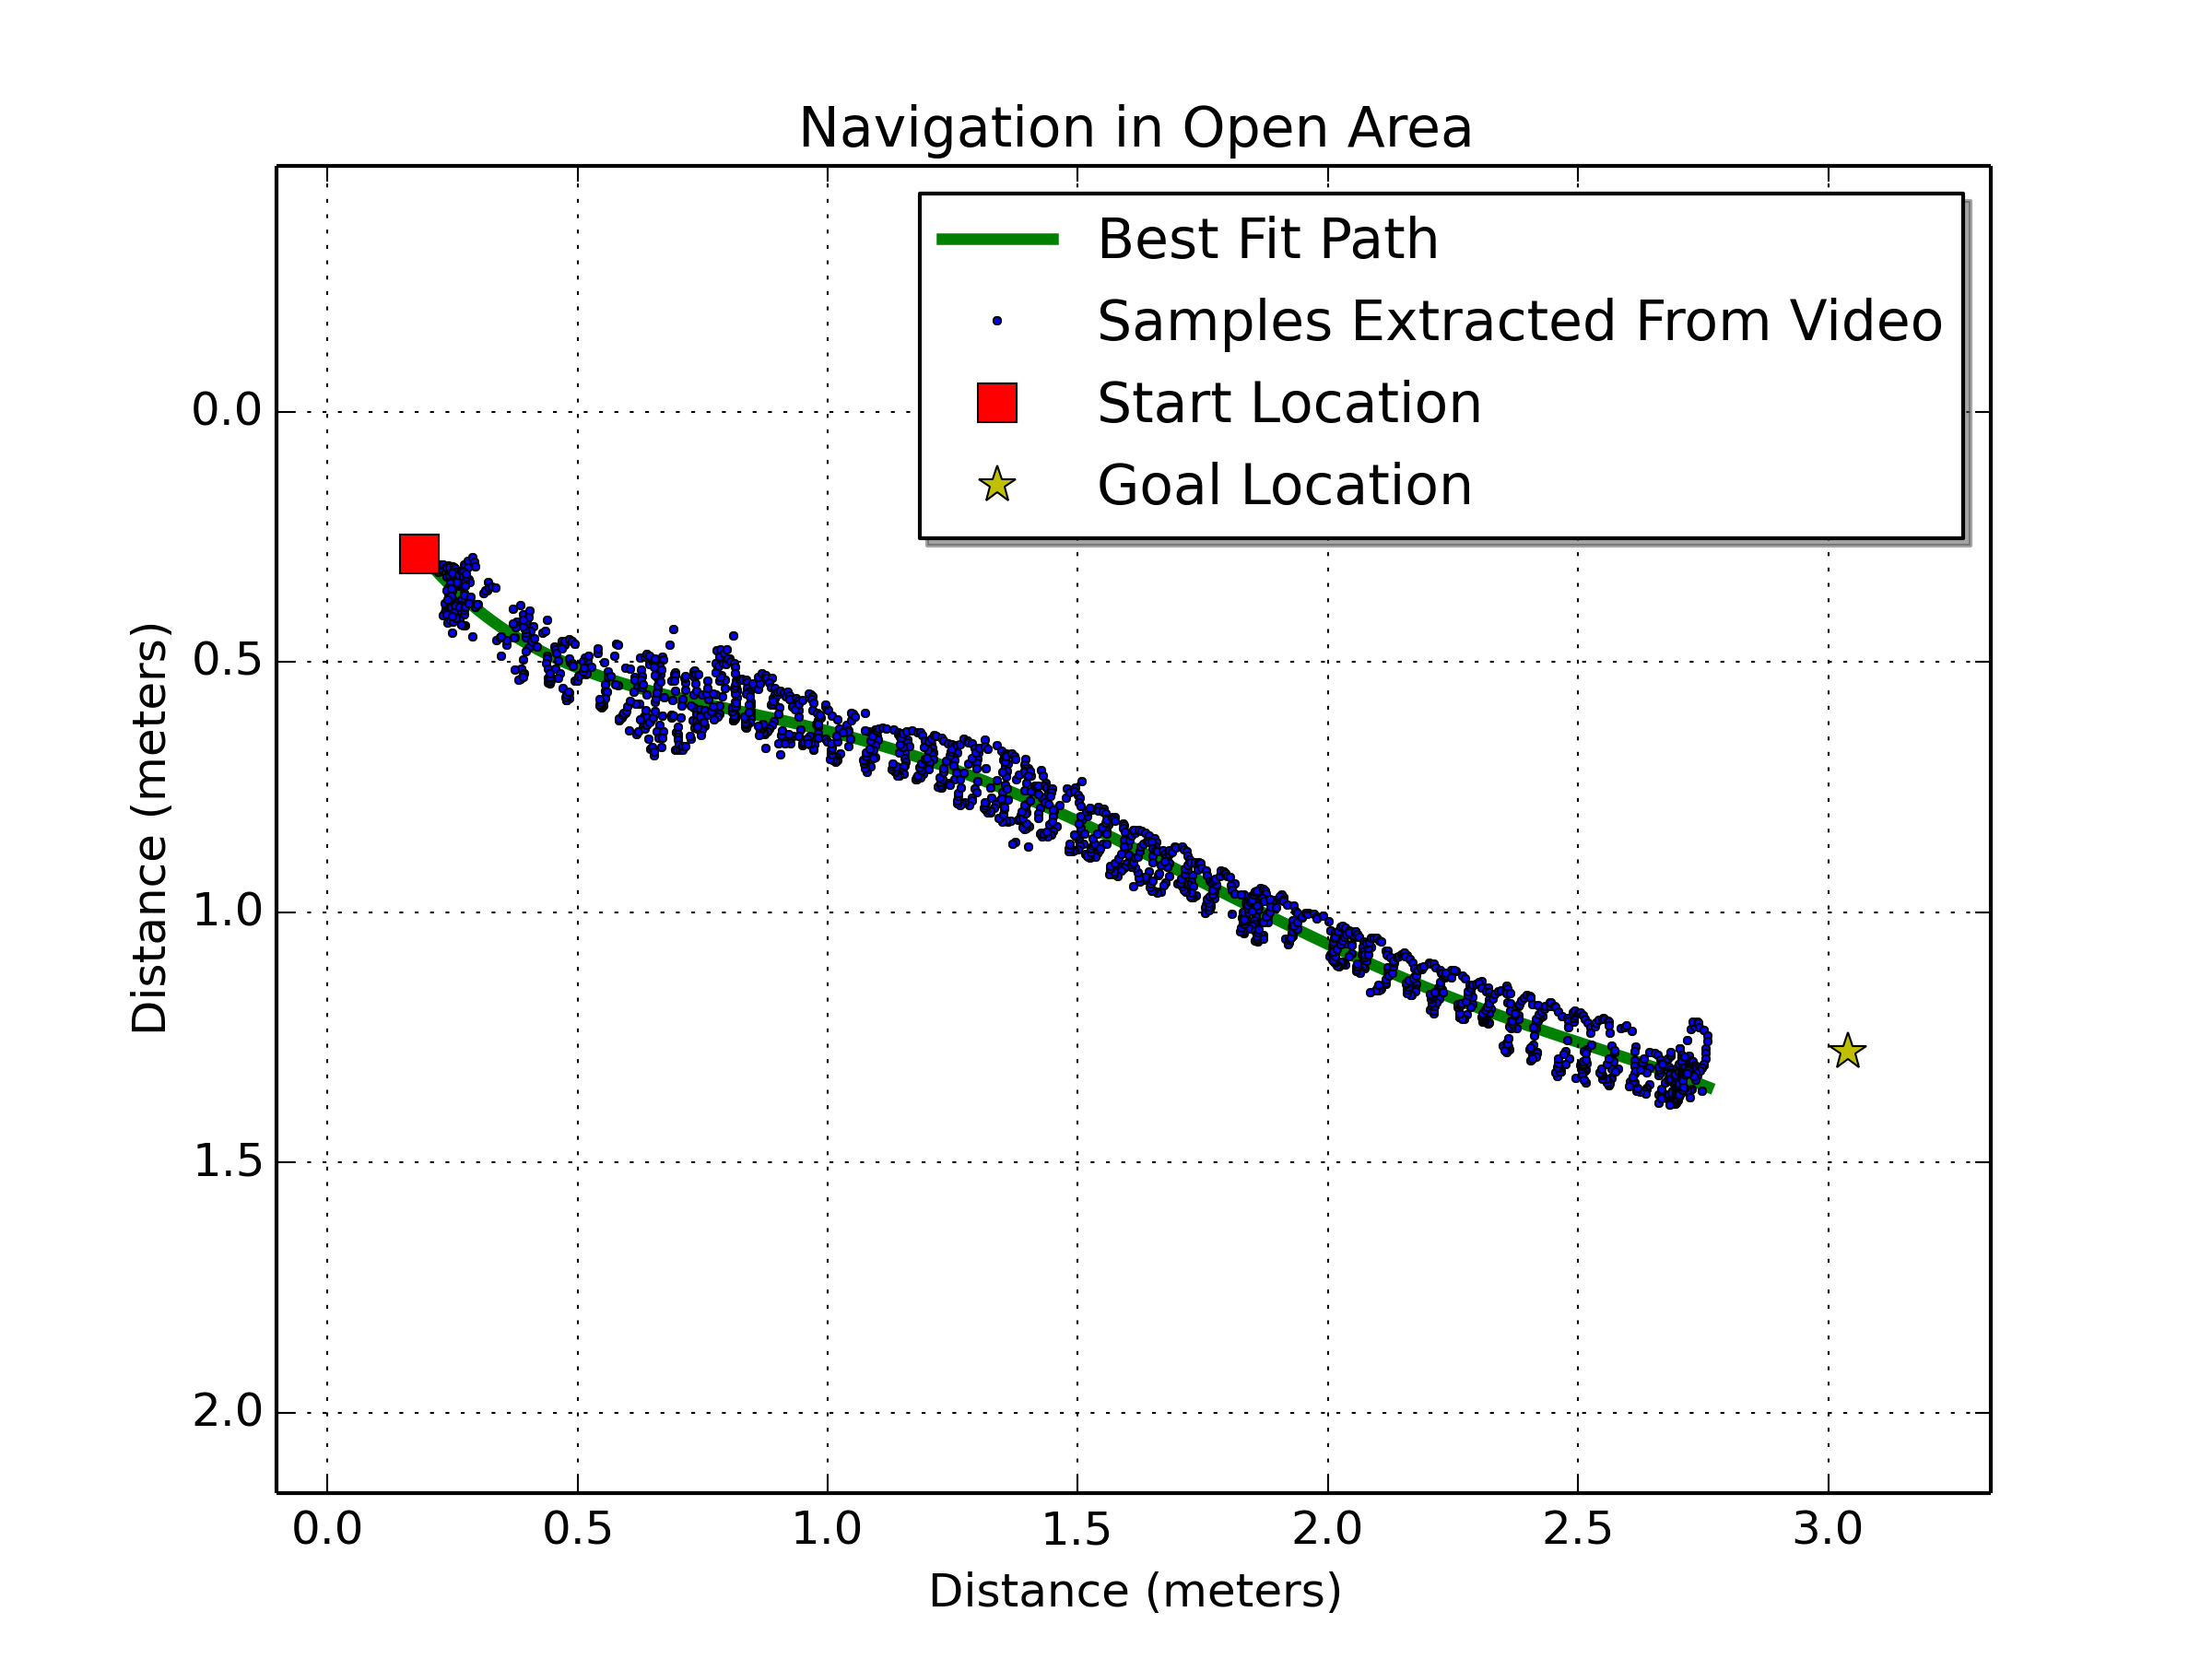
\includegraphics[height=0.5\textheight]{nav/open/plots/nav_open.png}
  \caption{Here's a plot of the robot as seen by the video and the best fit path, in the open area.
           You can really see the wobble here caused by the LIDAR + gait mismatch.
           The starting point is the red square on the left and the goal is the yellow star on the right.
           The robot was told to stop at some radius to the goal.}
  \label{fig:nav_open_plot1}
\end{figure}

\begin{figure}
  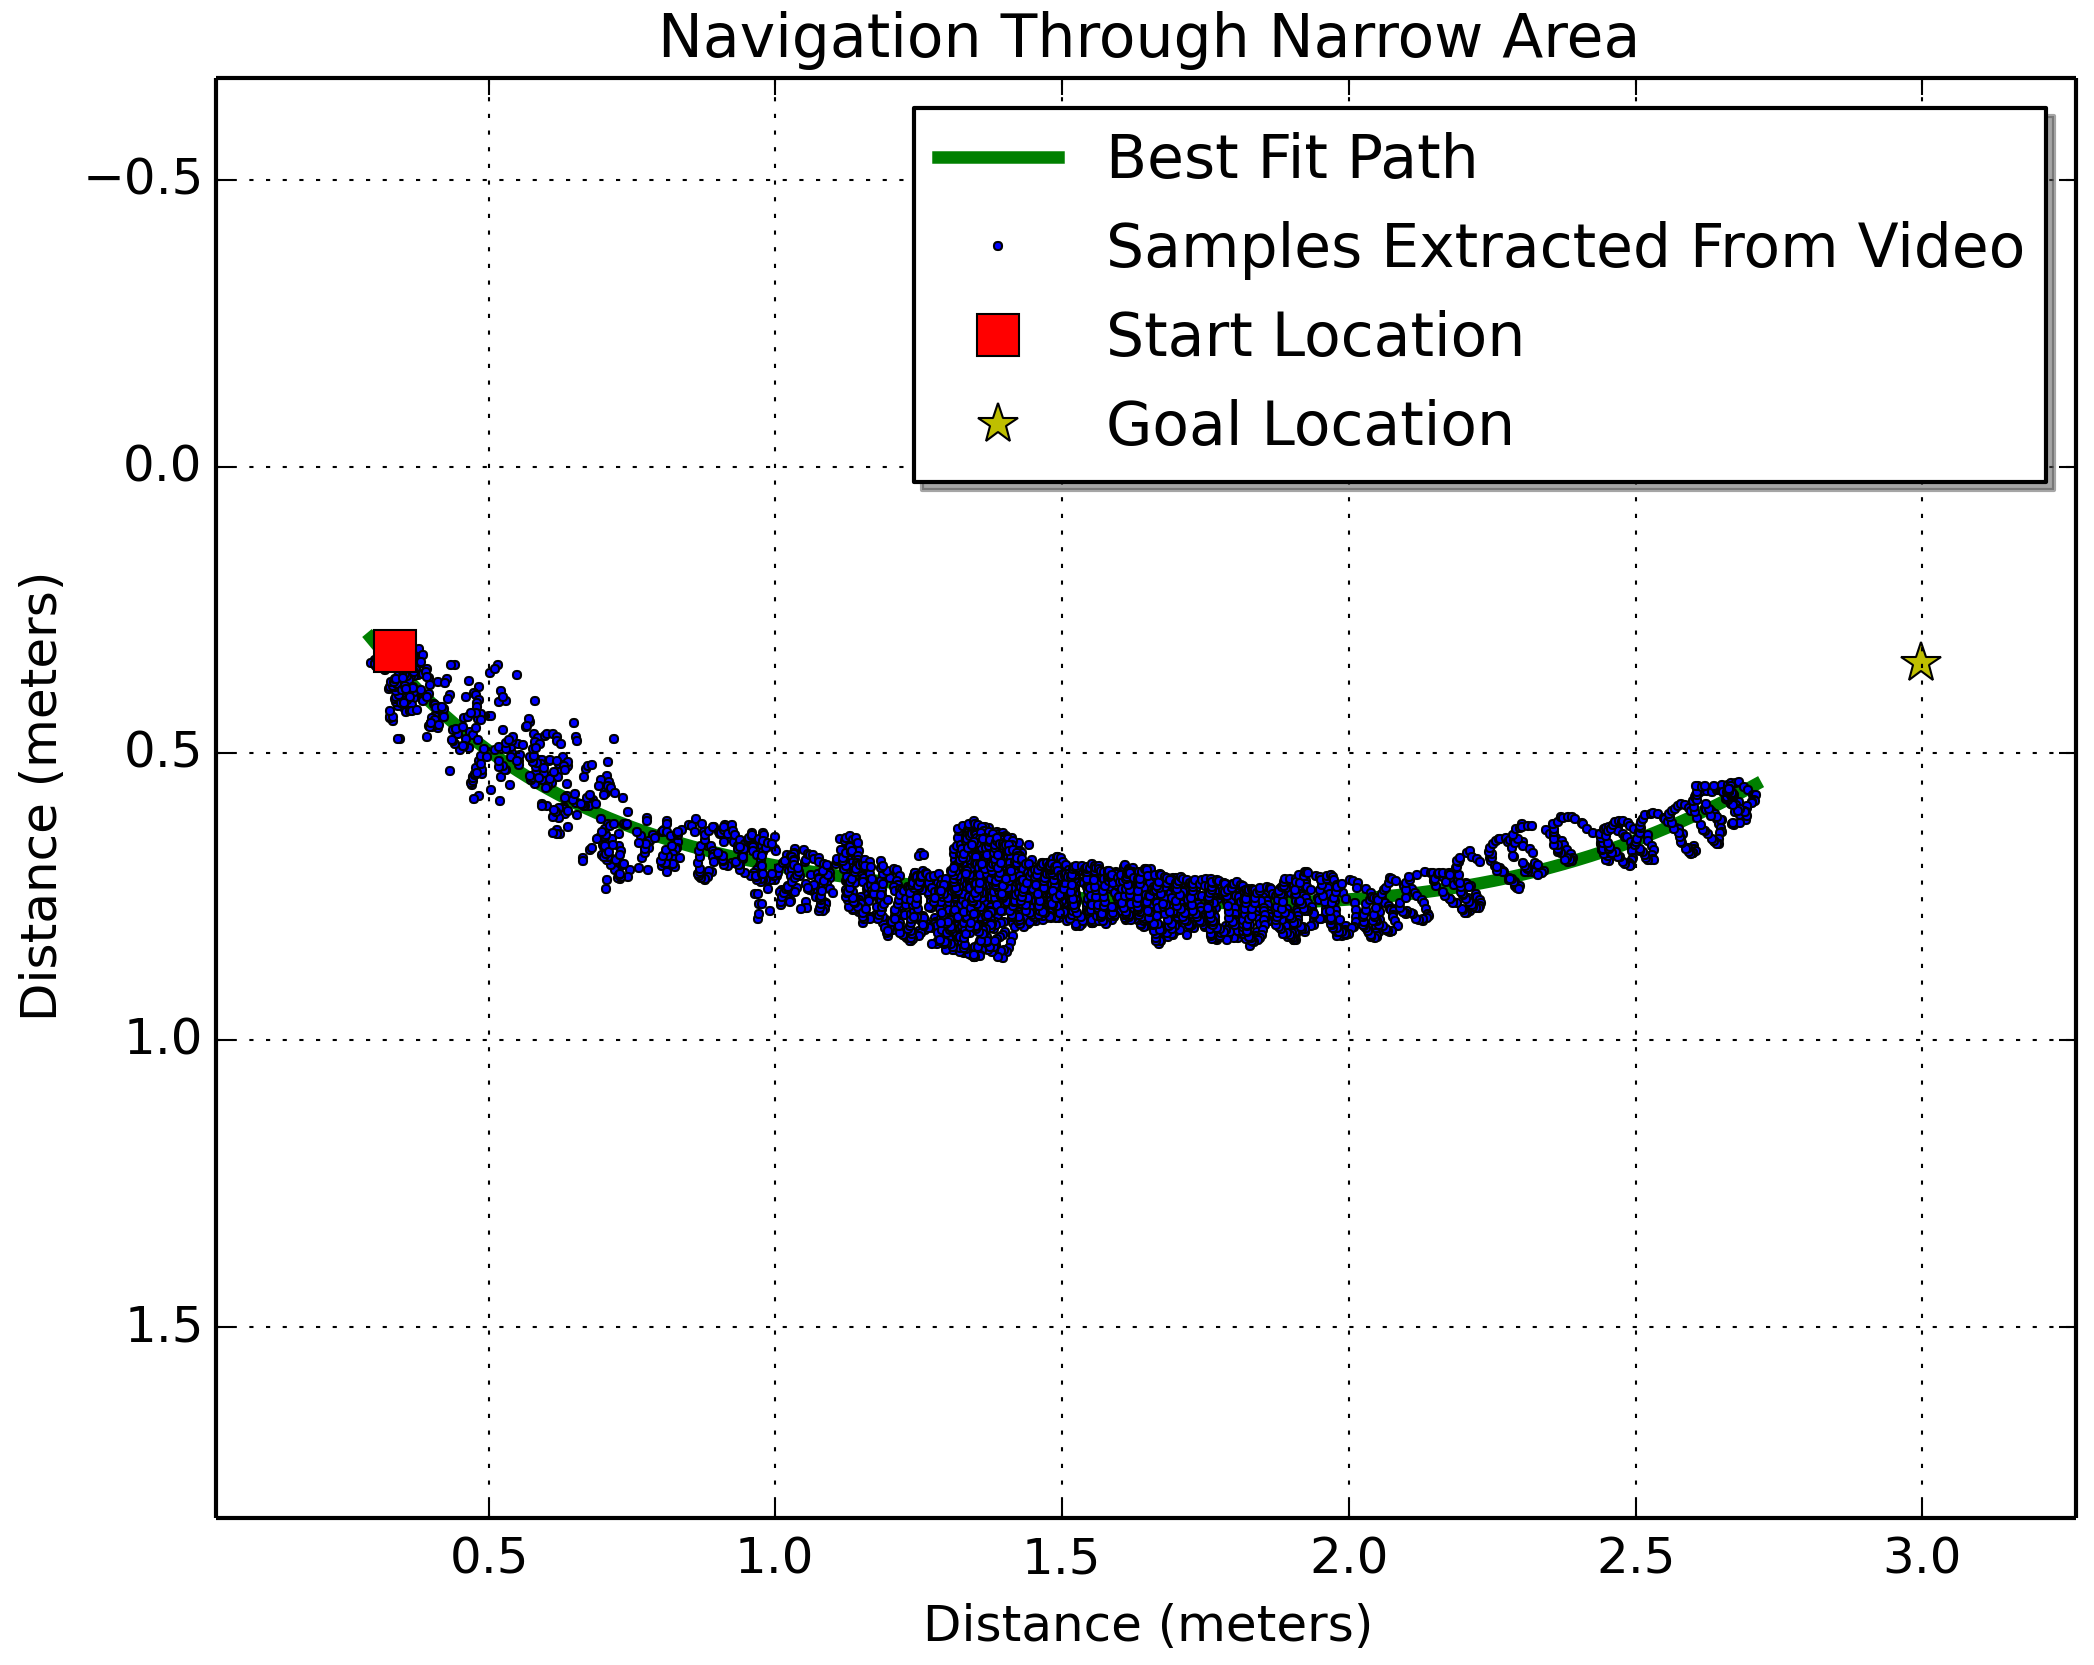
\includegraphics[height=0.5\textheight]{nav/narrow/plots/nav_narrow.png}
  \caption{Here's the plot of the robot walking through the narrow aperture.
           The robot had a lot of trouble at the opening of the aperture which can be seen by the
           large smattering of points in the $(1.4, 0.75)$ region. Again, this is because of
           the mismatch.}
  \label{fig:nav_narrow_plot1}
\end{figure}

\begin{figure}
  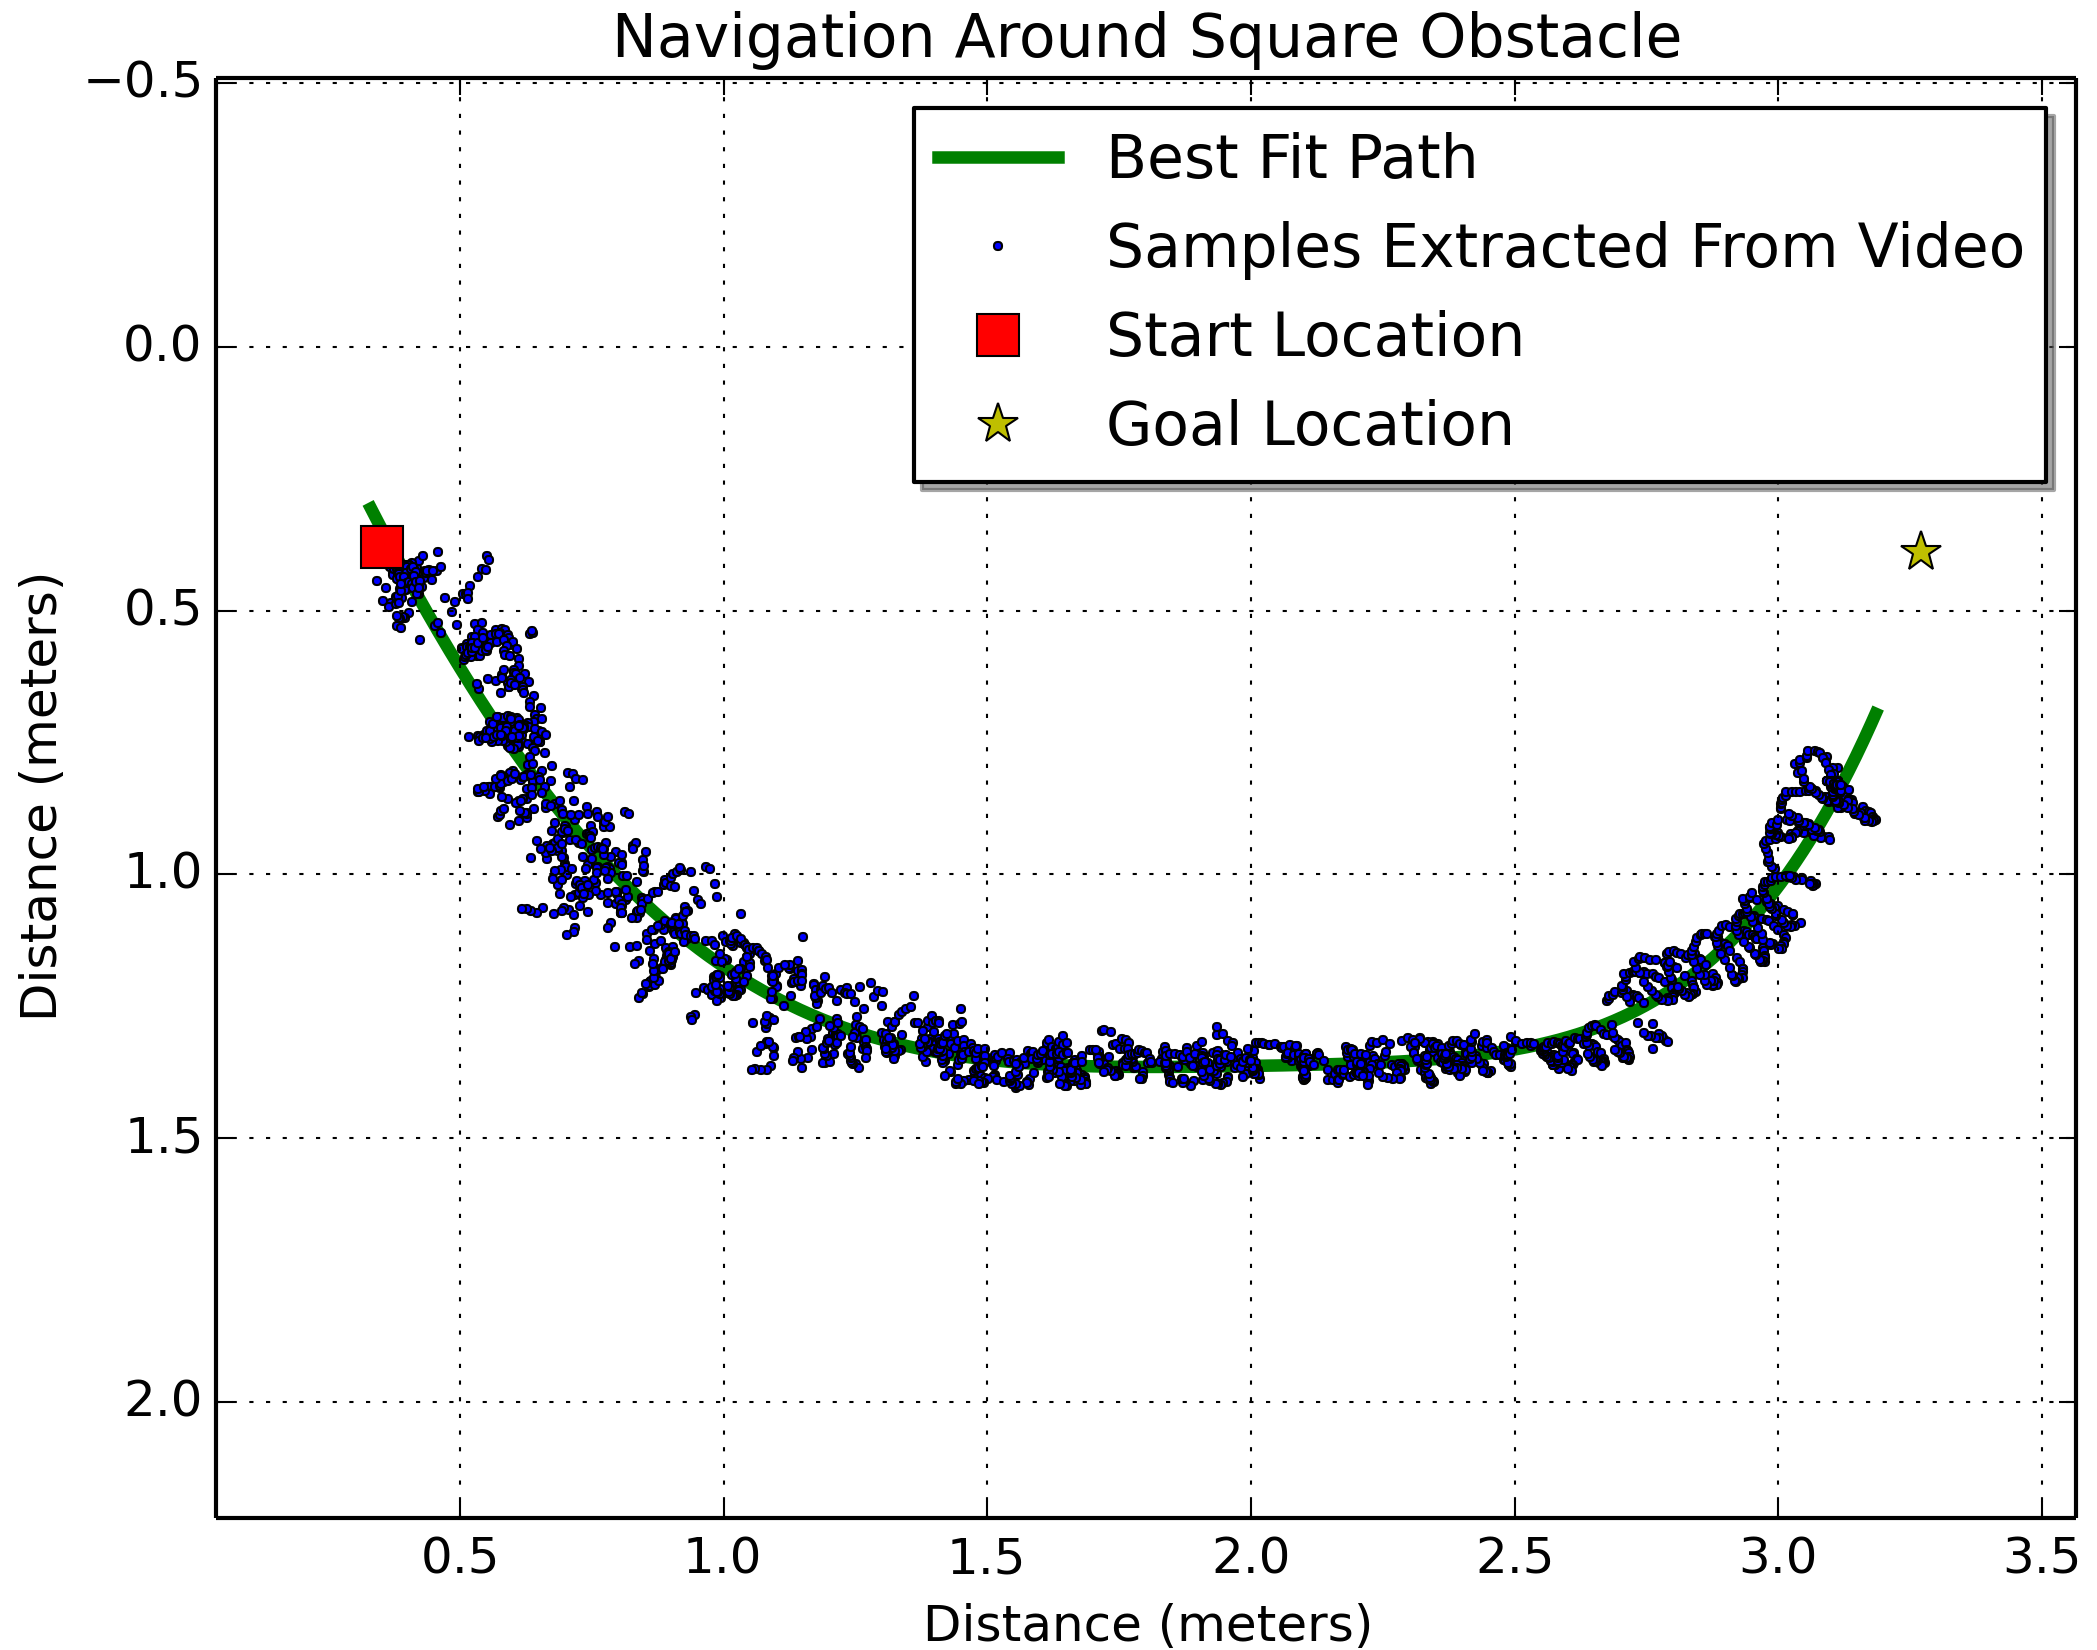
\includegraphics[height=0.5\textheight]{nav/square/plots/nav_square.png}
  \caption{Here's the plot of the robot walking around the square obstacle. It does pretty well.}
  \label{fig:nav_square_plot1}
\end{figure}

\section{What Nao Saw of the Goal}

I REALLY have no idea what these are suppose to do for you, but here they are.
This is what the Nao ``saw'' of the goal while it was walking.
The ranges are asymptotically decreasing like you would think they would do if the robot
was getting closer. This doesn't technically have to happen if the robot can ``slide''
along a straight wall for awhile where it could get a little longer for a bit or in a situation
where the range stays constant for awhile like a radial wall?
One thing to note is though that the range could never really increase significantly.
Like if the robot had to go around something that made it walk away, that would never happen.
The robot would be stuck in this local minima like we talked about in one of the sections of Chapter
\ref{ch:navigation}.
We'd have to use some sort of escape strategy.

The angle doesn't really tell you much since it's the relative bearing which is important to the robot
but hard for use to interpret since we don't know the global orientation of the robot.
Actually, since the goal is not moving, then we probably could do better with the orientation data
to tell us the orientation of the robot. It's not worth it for this thesis but we could run it through
some filters and get something to work. We'd either have to EKF it with the initial pose or PF it.
Not really part of the thesis, but then it makes sense to have analyzed the data because then we could
use it as the ground truth for a localization algorithm (like Agraj did).
The best we can say is that in one of them (the open area one which makes sense since it had plenty of
time to get a lock on things and ride the pipe in) it's like always decreasing so he's homing in on things
and in the others it's oscillating back and forth so it's marginally stable or
looks like it's some other type of stability like lyapunov or some other thing, which you could
say means he's got a good track on things.

I mentioned before that the robot was commanded to stop at 0.3 meters but actually stops closer
to 0.8 meters because of the perception mismatch.
In the figures \ref{fig:nav_open_rb1}, \ref{fig:nav_narrow_rb1}, and \ref{fig:nav_square_rb1},
you can see that the robot thinks it's stopping at the appropriate distance
of 0.3 meters.

\begin{figure}
  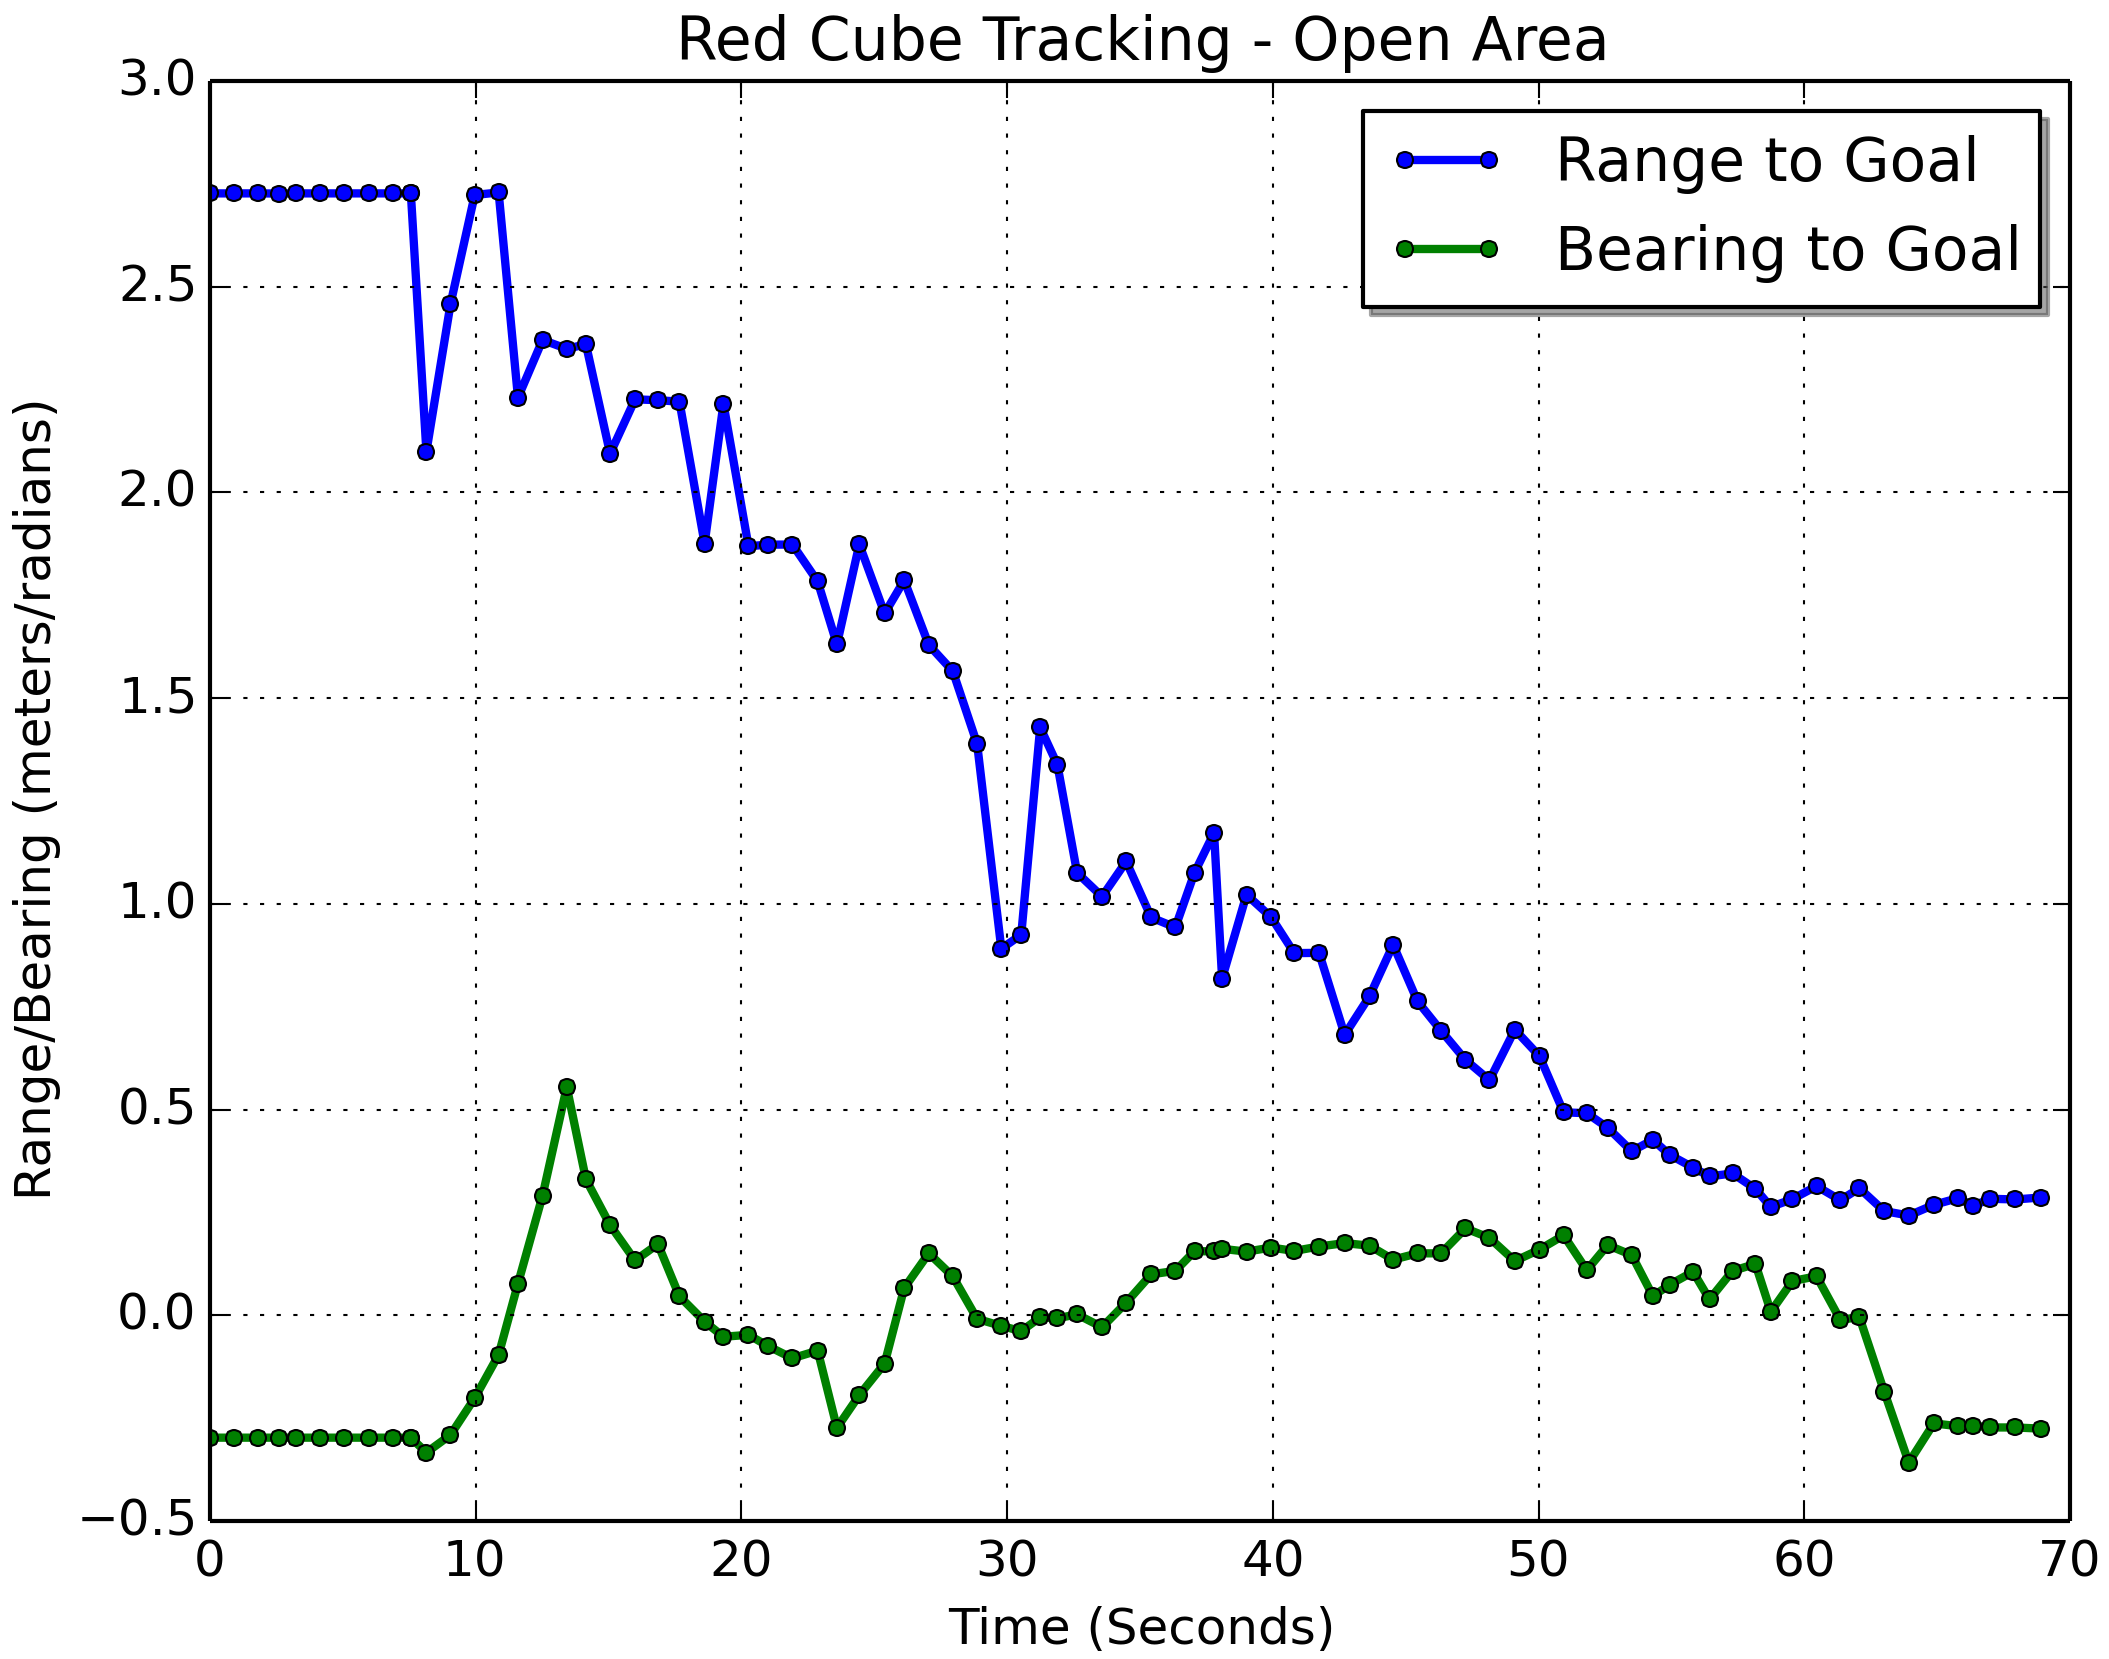
\includegraphics[height=0.5\textheight]{nav/open/tracking/open_rb1.png}
  \caption{This is what the robot saw in the open area.
           The range decreased like you'd expect and the bearing is basically working its way
           to convergence for a lot of it because the robot had time to do so.}
  \label{fig:nav_open_rb1}
\end{figure}

\begin{figure}
  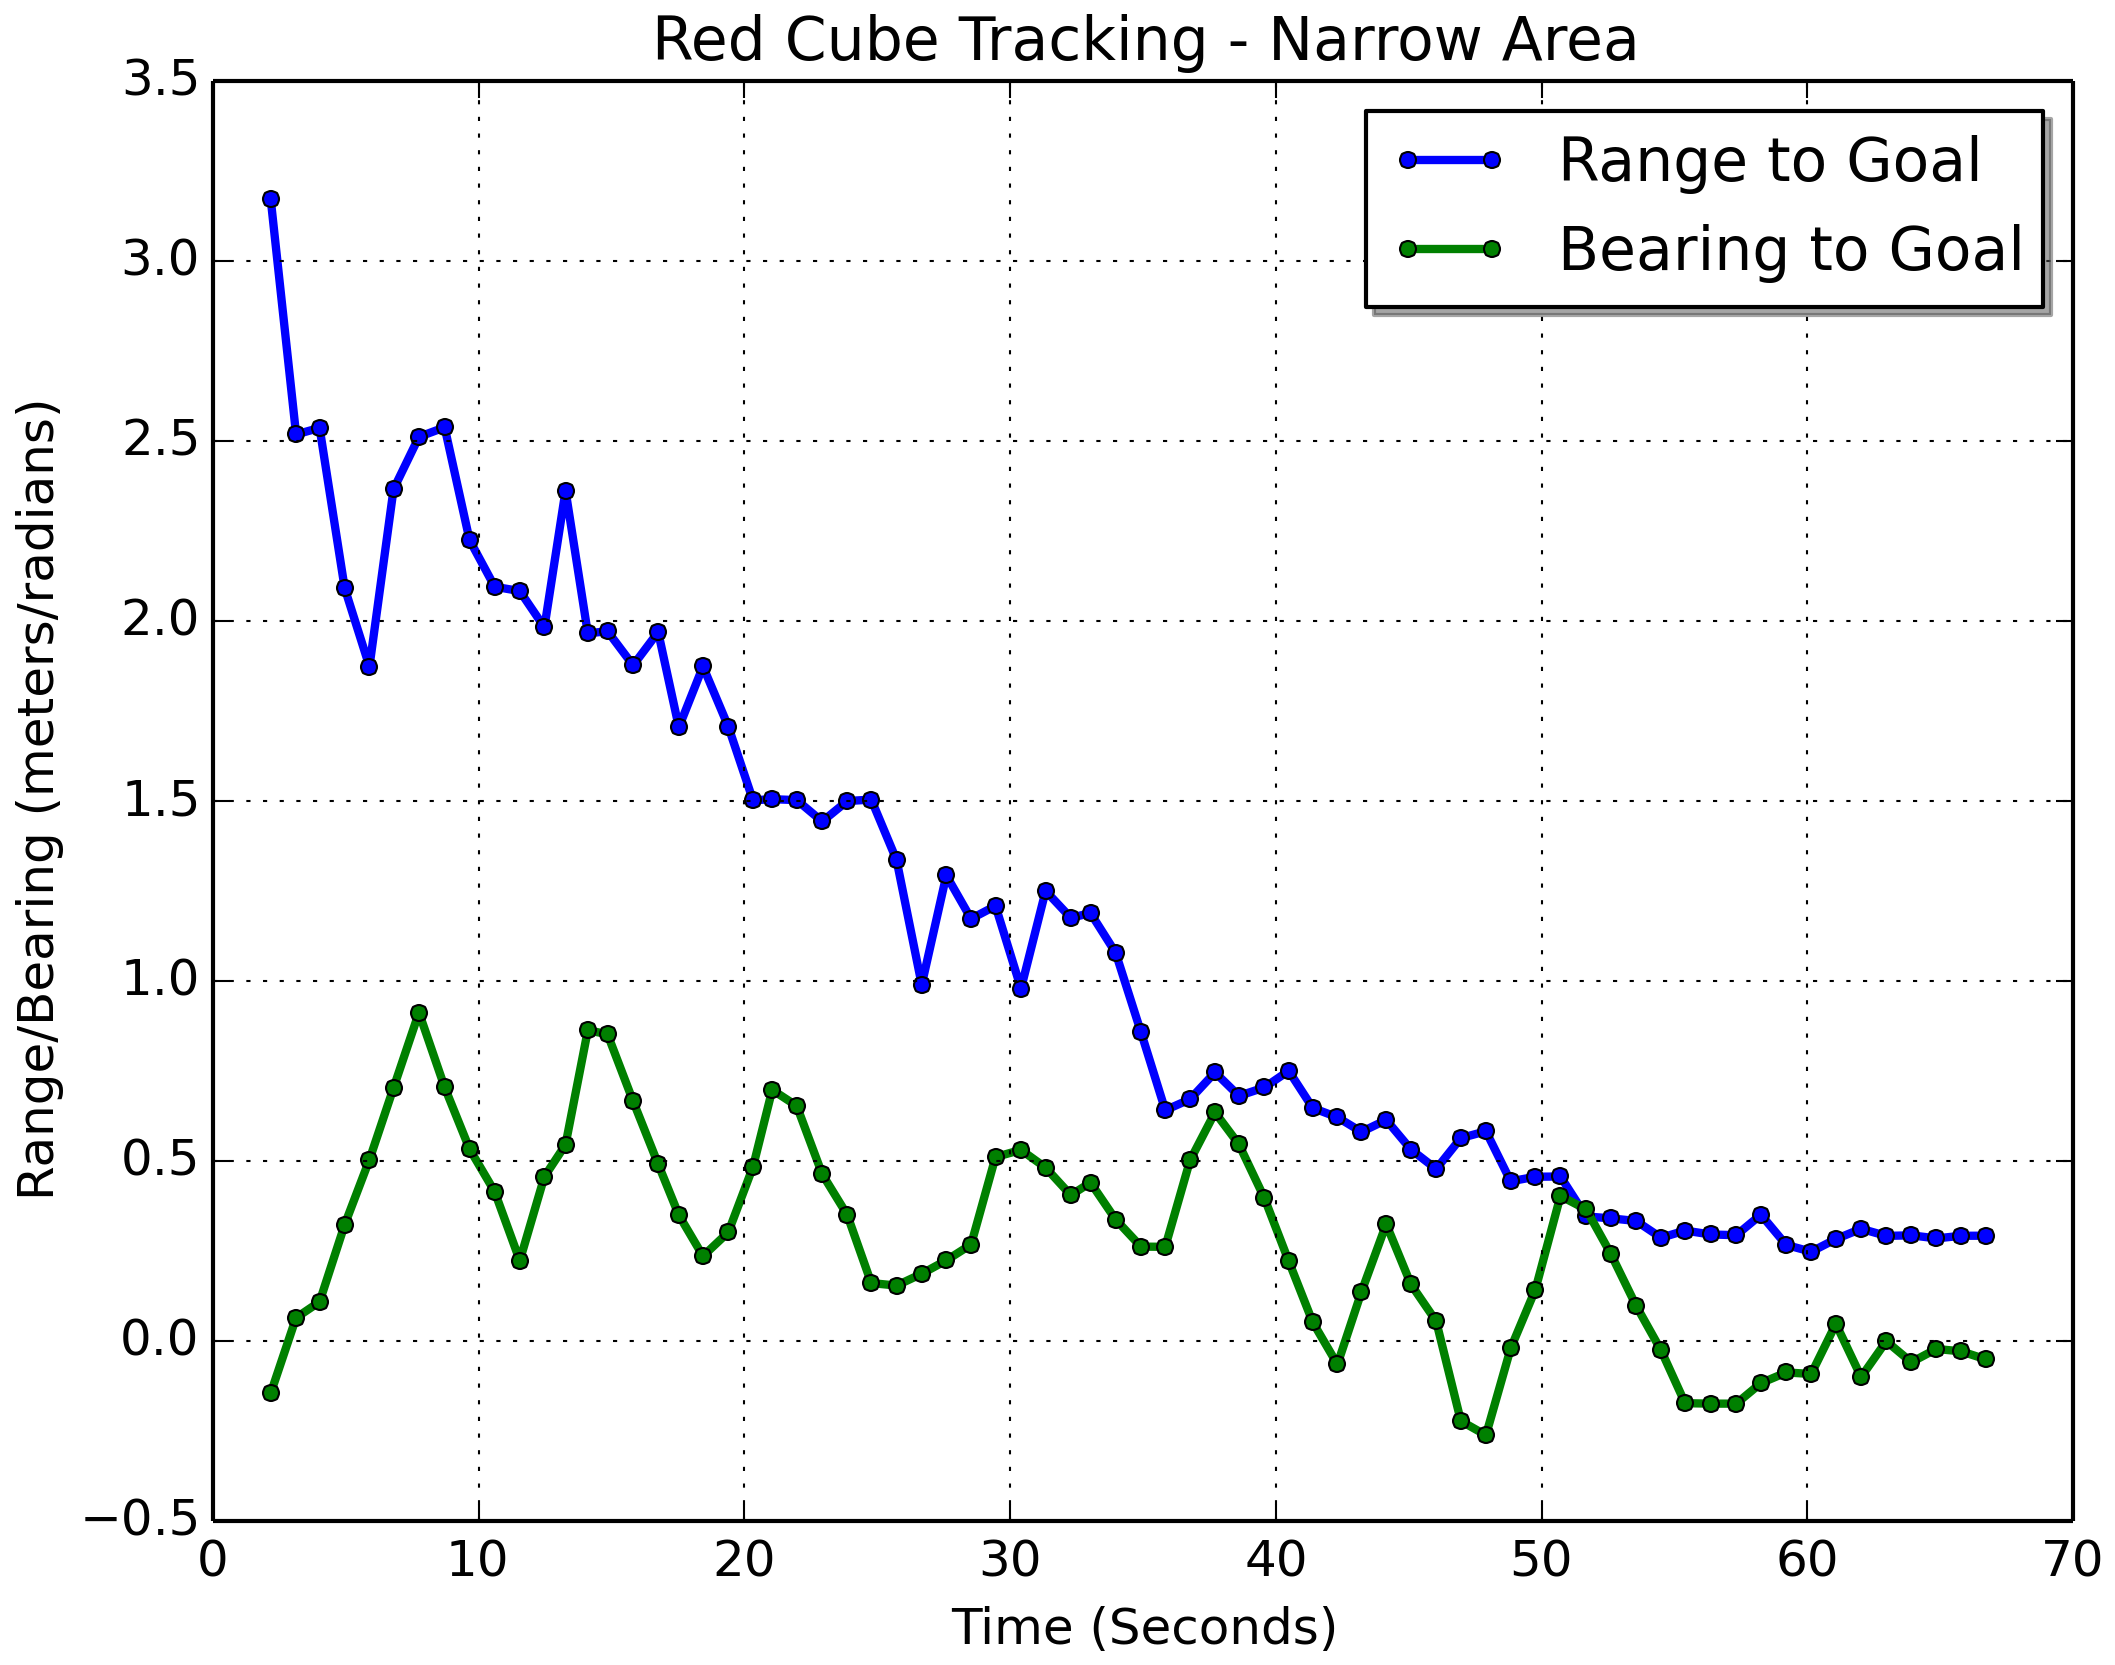
\includegraphics[height=0.5\textheight]{nav/narrow/tracking/narrow_rb1.png}
  \caption{Here's what the robot saw during the narrow aperture run.
           Again, the range decreases but the bearing doesn't.
           This is fine because the robot is moving and turning and stuff so the bearing
           won't really converge.}
  \label{fig:nav_narrow_rb1}
\end{figure}

\begin{figure}
  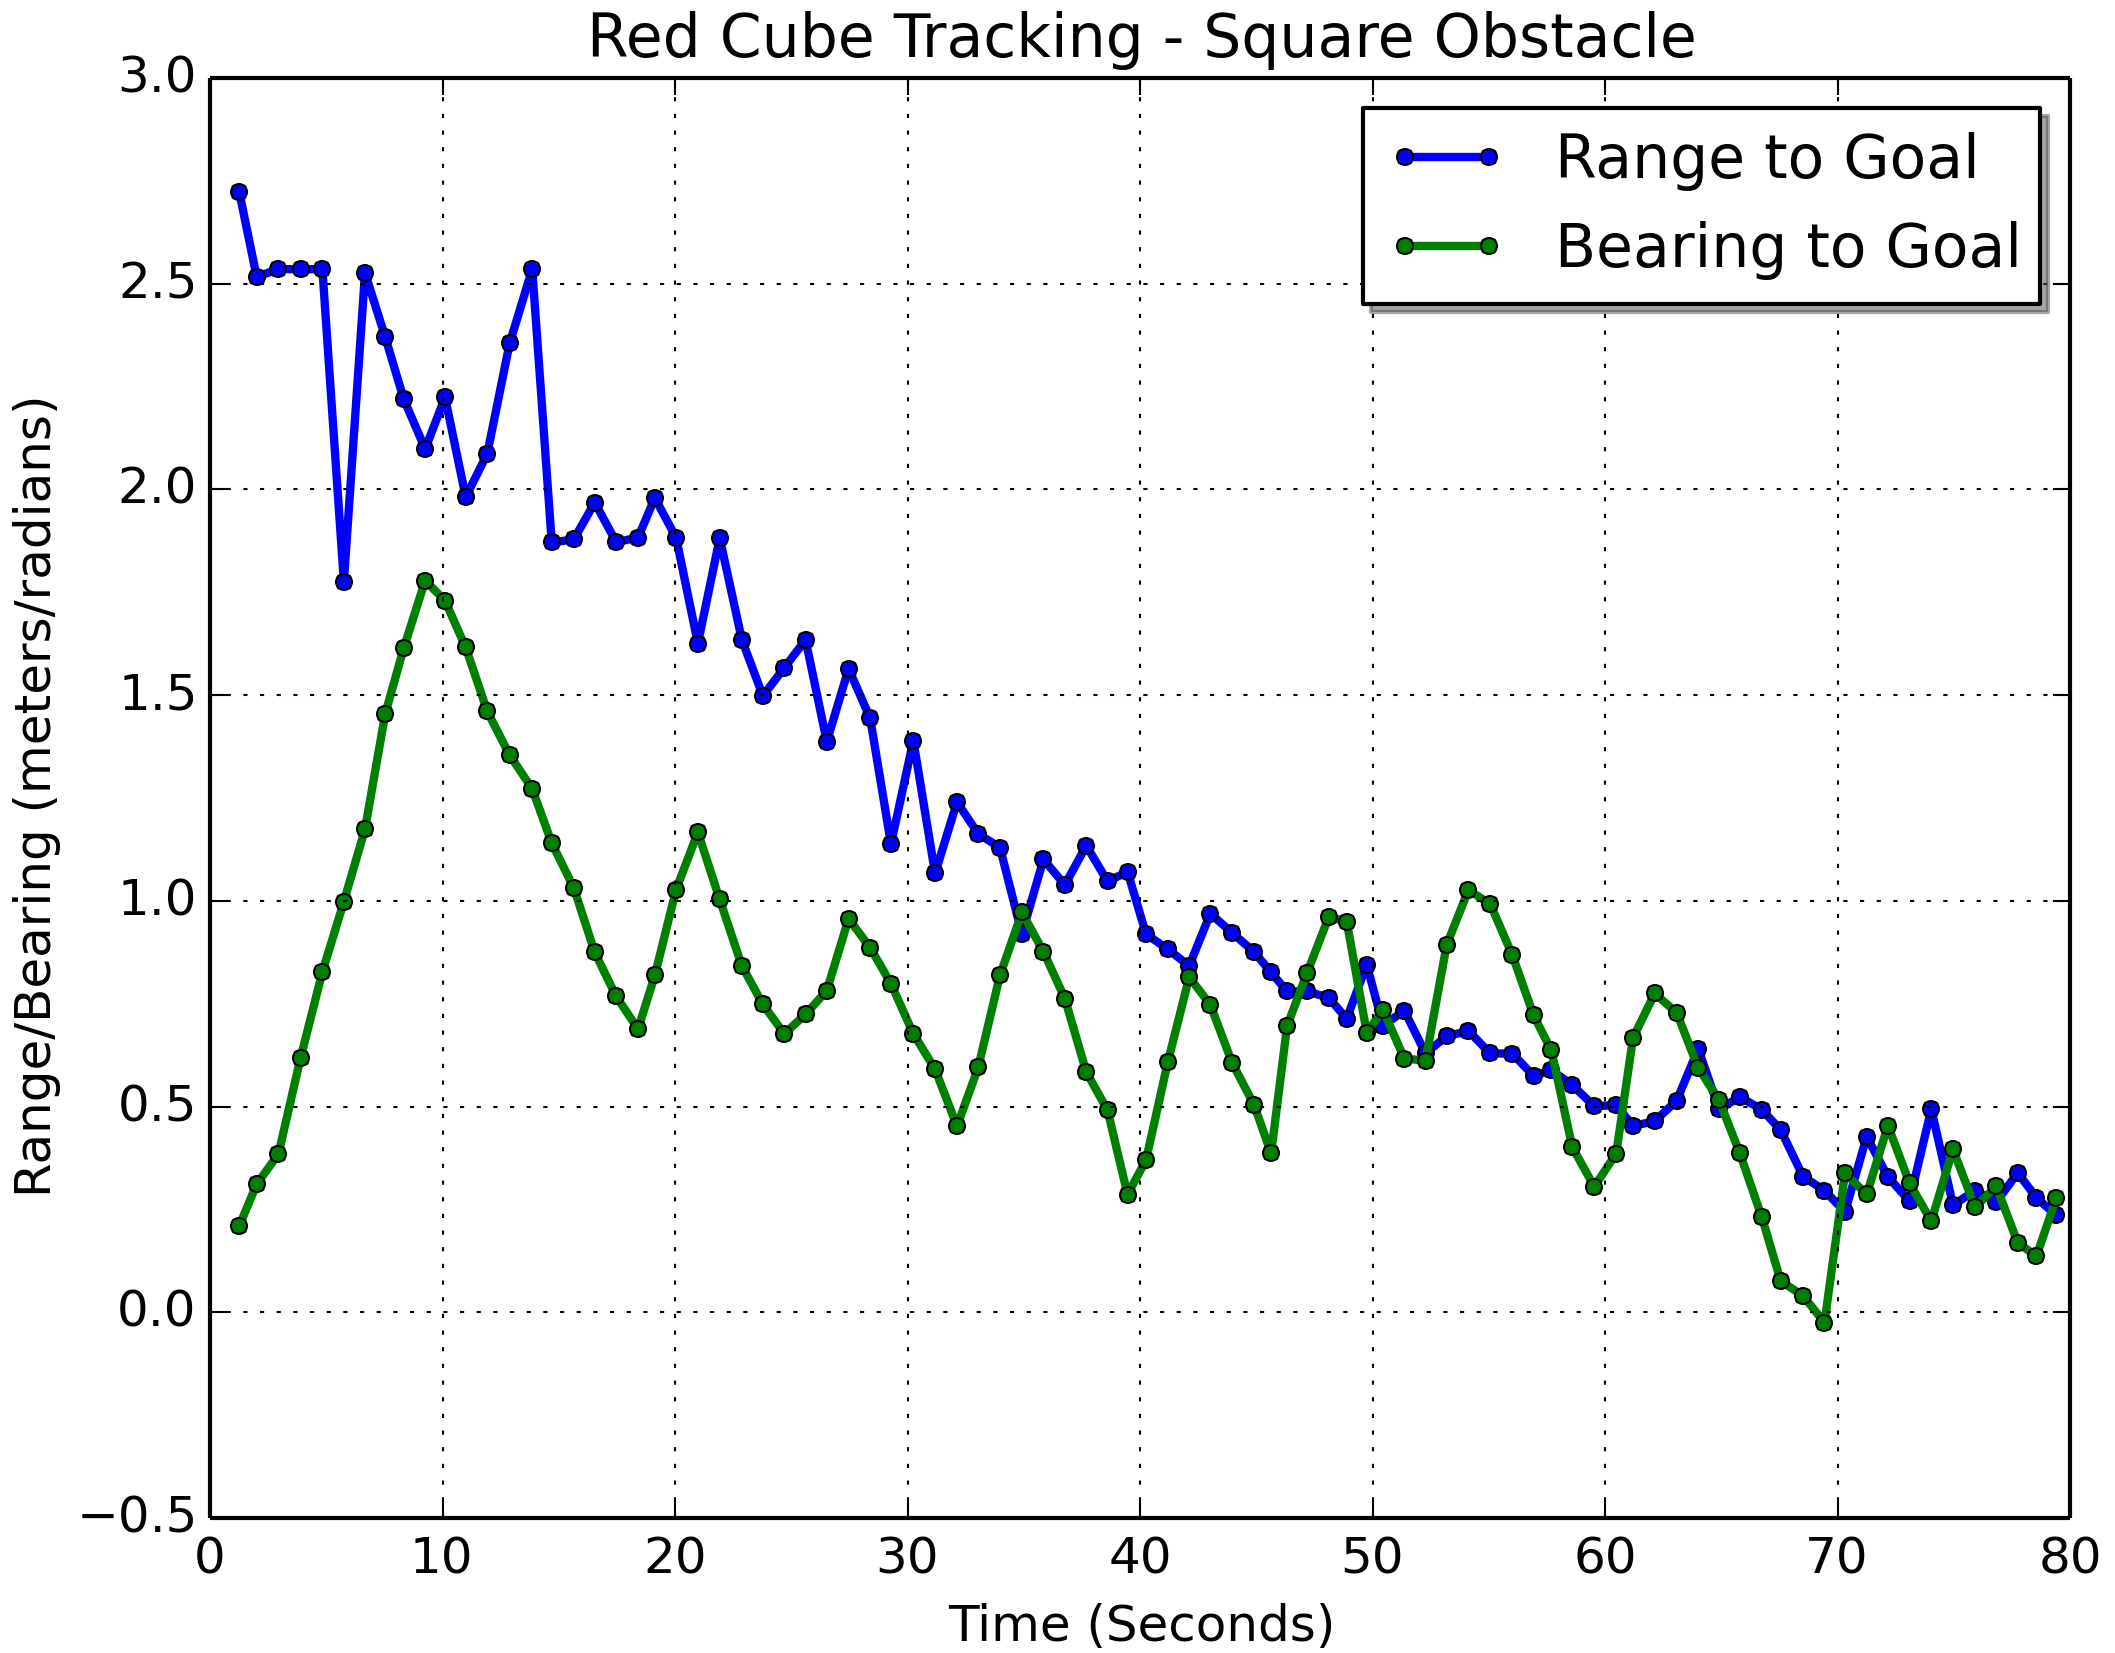
\includegraphics[height=0.5\textheight]{nav/square/tracking/square_rb1.png}
  \caption{This is what the robot saw during the large obstacle run.
           It basically has the same behavior as the other one.}
  \label{fig:nav_square_rb1}
\end{figure}